% Options for packages loaded elsewhere
\PassOptionsToPackage{unicode}{hyperref}
\PassOptionsToPackage{hyphens}{url}
\PassOptionsToPackage{dvipsnames,svgnames,x11names}{xcolor}
%
\documentclass[
  article]{jss}

\usepackage{amsmath,amssymb}
\usepackage{iftex}
\ifPDFTeX
  \usepackage[T1]{fontenc}
  \usepackage[utf8]{inputenc}
  \usepackage{textcomp} % provide euro and other symbols
\else % if luatex or xetex
  \usepackage{unicode-math}
  \defaultfontfeatures{Scale=MatchLowercase}
  \defaultfontfeatures[\rmfamily]{Ligatures=TeX,Scale=1}
\fi
\usepackage{lmodern}
\ifPDFTeX\else  
    % xetex/luatex font selection
\fi
% Use upquote if available, for straight quotes in verbatim environments
\IfFileExists{upquote.sty}{\usepackage{upquote}}{}
\IfFileExists{microtype.sty}{% use microtype if available
  \usepackage[]{microtype}
  \UseMicrotypeSet[protrusion]{basicmath} % disable protrusion for tt fonts
}{}
\makeatletter
\@ifundefined{KOMAClassName}{% if non-KOMA class
  \IfFileExists{parskip.sty}{%
    \usepackage{parskip}
  }{% else
    \setlength{\parindent}{0pt}
    \setlength{\parskip}{6pt plus 2pt minus 1pt}}
}{% if KOMA class
  \KOMAoptions{parskip=half}}
\makeatother
\usepackage{xcolor}
\setlength{\emergencystretch}{3em} % prevent overfull lines
\setcounter{secnumdepth}{-\maxdimen} % remove section numbering
% Make \paragraph and \subparagraph free-standing
\ifx\paragraph\undefined\else
  \let\oldparagraph\paragraph
  \renewcommand{\paragraph}[1]{\oldparagraph{#1}\mbox{}}
\fi
\ifx\subparagraph\undefined\else
  \let\oldsubparagraph\subparagraph
  \renewcommand{\subparagraph}[1]{\oldsubparagraph{#1}\mbox{}}
\fi


\providecommand{\tightlist}{%
  \setlength{\itemsep}{0pt}\setlength{\parskip}{0pt}}\usepackage{longtable,booktabs,array}
\usepackage{calc} % for calculating minipage widths
% Correct order of tables after \paragraph or \subparagraph
\usepackage{etoolbox}
\makeatletter
\patchcmd\longtable{\par}{\if@noskipsec\mbox{}\fi\par}{}{}
\makeatother
% Allow footnotes in longtable head/foot
\IfFileExists{footnotehyper.sty}{\usepackage{footnotehyper}}{\usepackage{footnote}}
\makesavenoteenv{longtable}
\usepackage{graphicx}
\makeatletter
\def\maxwidth{\ifdim\Gin@nat@width>\linewidth\linewidth\else\Gin@nat@width\fi}
\def\maxheight{\ifdim\Gin@nat@height>\textheight\textheight\else\Gin@nat@height\fi}
\makeatother
% Scale images if necessary, so that they will not overflow the page
% margins by default, and it is still possible to overwrite the defaults
% using explicit options in \includegraphics[width, height, ...]{}
\setkeys{Gin}{width=\maxwidth,height=\maxheight,keepaspectratio}
% Set default figure placement to htbp
\makeatletter
\def\fps@figure{htbp}
\makeatother

\usepackage{orcidlink,thumbpdf,lmodern}

\newcommand{\class}[1]{`\code{#1}'}
\newcommand{\fct}[1]{\code{#1()}}
\makeatletter
\makeatother
\makeatletter
\makeatother
\makeatletter
\@ifpackageloaded{caption}{}{\usepackage{caption}}
\AtBeginDocument{%
\ifdefined\contentsname
  \renewcommand*\contentsname{Table of contents}
\else
  \newcommand\contentsname{Table of contents}
\fi
\ifdefined\listfigurename
  \renewcommand*\listfigurename{List of Figures}
\else
  \newcommand\listfigurename{List of Figures}
\fi
\ifdefined\listtablename
  \renewcommand*\listtablename{List of Tables}
\else
  \newcommand\listtablename{List of Tables}
\fi
\ifdefined\figurename
  \renewcommand*\figurename{Figure}
\else
  \newcommand\figurename{Figure}
\fi
\ifdefined\tablename
  \renewcommand*\tablename{Table}
\else
  \newcommand\tablename{Table}
\fi
}
\@ifpackageloaded{float}{}{\usepackage{float}}
\floatstyle{ruled}
\@ifundefined{c@chapter}{\newfloat{codelisting}{h}{lop}}{\newfloat{codelisting}{h}{lop}[chapter]}
\floatname{codelisting}{Listing}
\newcommand*\listoflistings{\listof{codelisting}{List of Listings}}
\makeatother
\makeatletter
\@ifpackageloaded{caption}{}{\usepackage{caption}}
\@ifpackageloaded{subcaption}{}{\usepackage{subcaption}}
\makeatother
\makeatletter
\makeatother
\ifLuaTeX
  \usepackage{selnolig}  % disable illegal ligatures
\fi
\IfFileExists{bookmark.sty}{\usepackage{bookmark}}{\usepackage{hyperref}}
\IfFileExists{xurl.sty}{\usepackage{xurl}}{} % add URL line breaks if available
\urlstyle{same} % disable monospaced font for URLs
\hypersetup{
  pdftitle={Team 15 The Scientists: Crime Prediction Proposal},
  pdfauthor={Xiangyu Jin (xjin13); Vinayak Bagdi (vbagdi2)},
  pdfkeywords={R, group project},
  colorlinks=true,
  linkcolor={blue},
  filecolor={Maroon},
  citecolor={Blue},
  urlcolor={Blue},
  pdfcreator={LaTeX via pandoc}}

%% -- Article metainformation (author, title, ...) -----------------------------

%% Author information
\author{Xiangyu Jin (xjin13)\\UIUC \And Vinayak Bagdi (vbagdi2)\\UIUC}
\Plainauthor{Xiangyu Jin (xjin13), Vinayak Bagdi
(vbagdi2)} %% comma-separated

\title{Team 15 The Scientists: Crime Prediction Proposal}
\Plaintitle{Team 15 The Scientists: Crime Prediction
Proposal} %% without formatting

%% an abstract and keywords
\Abstract{The project aims to predict the type of crime an arrestee may
have committed based on their background information such as race, sex,
age, and other attributes. The central idea is to examine whether there
are any relationships between crime types and arrestee's background
information and to study the crime distribution in Champaign The project
employs classification models or random forests model to predict the
crime type based on the information about the arrestees. The project
uses data before 2018 as training data and data after 2018 as testing
data to test the model's accuracy. The methods employed so far include
data cleaning, feature engineering, data manipulation, data
visualization, and data analysis using R. The implications of the work
done so far will help to improve the understanding of crime distribution
in Champaign and aid in the development of effective crime prevention
and control strategies.}

%% at least one keyword must be supplied
\Keywords{R, group project}
\Plainkeywords{R, group project}

%% publication information
%% NOTE: Typically, this can be left commented and will be filled out by the technical editor
%% \Volume{50}
%% \Issue{9}
%% \Month{June}
%% \Year{2012}
%% \Submitdate{2012-06-04}
%% \Acceptdate{2012-06-04}
%% \setcounter{page}{1}
%% \Pages{1--xx}

%% The address of (at least) one author should be given
%% in the following format:
\Address{
Xiangyu Jin (xjin13)\\
Department of Statistics\\
E-mail: \email{xjin13@illinois.edu}\\
\\~
Vinayak Bagdi (vbagdi2)\\
Department of Statistics\\
E-mail: \email{vbagdi2@illinois.edu}\\
\\~

}

\begin{document}
\maketitle
\hypertarget{introduction}{%
\subsection{Introduction}\label{introduction}}

The project aims to examine the relationship between the type of crime
and the background information of the arrestees, including race, sex,
age, and other attributes. The problem being addressed is the high rate
of crime in Champaign, which poses a significant threat to the safety
and well-being of residents. It is essential to develop effective crime
prevention and control strategies that take into account the underlying
factors contributing to crime. The objective of the project is to
predict the type of crime an arrestee may have committed based on their
background information, which can aid in developing effective crime
prevention strategies.

The motivation for pursuing this problem is to improve the understanding
of crime distribution in Champaign and to identify potential factors
contributing to the high rate of crime. The project can aid in the
development of targeted crime prevention and control strategies that can
help to reduce crime rates in the city. Additionally, the project can
help law enforcement agencies to allocate resources effectively and
efficiently.

\hypertarget{related-works}{%
\subsection{Related Works}\label{related-works}}

\citet{Travaini2022} explores the use of machine learning algorithms to
predict the likelihood of criminal recidivism. The study used a dataset
consisting of demographic and criminal history variables of inmates to
develop a prediction model. This study is relevant to our project as it
also uses machine learning algorithms to predict criminal activities
based on input features. However, the focus of our project is on
predicting the type of crime based on the background information of the
arrestees, whereas the study by \citet{Travaini2022} is focused on
predicting the likelihood of criminal recidivism. Both employ machine
learning algorithms to predict criminal activities based on input
features. However, the input features and prediction targets are
different. Our project focuses on predicting the type of crime based on
the background information of the arrestees, whereas the study by
\citet{Travaini2022} focuses on predicting the likelihood of criminal
recidivism based on demographic and criminal history variables of
inmates.

\citet{Saeed2015} explores the use of machine learning algorithms to
classify criminal activities based on the input features. The study used
a dataset consisting of demographic and behavioral variables of
criminals to develop a prediction model.This study is relevant to the
current project as it also uses machine learning algorithms to predict
criminal activities based on input features. The focus of our project is
on predicting the type of crime based on the background information of
the arrestees, whereas the study by \citet{Saeed2015} is focused on
classifying criminal activities based on the input features. Both employ
machine learning algorithms to predict criminal activities based on
input features. However, the prediction targets are different. Our
project focuses on predicting the type of crime based on the background
information of the arrestees, whereas the study by \citet{Saeed2015}
focuses on classifying criminal activities based on the input features.

\citet{Mandalapu2023} is a systematic review of crime prediction using
machine learning techniques. The authors reviewed and analyzed 82
research papers from 2010 to 2019. The review highlights the importance
of data preprocessing, feature selection, and algorithm selection in
crime prediction. The authors also discuss the limitations and
challenges of using machine learning in crime prediction, such as data
imbalance, interpretability, and ethical concerns. This work relates to
our current project as it provides insights into the state of the art in
crime prediction using machine learning techniques. It highlights the
importance of data preprocessing and algorithm selection, which are
critical steps in our project. It also discusses the challenges and
limitations of using machine learning in crime prediction, which we
should be aware of when interpreting our results. Our approach will be
similar to the reviewed papers in terms of using machine learning
techniques for crime prediction. However, we will focus on a specific
dataset from Champaign and investigate the relationship between crime
types and arrestee's background information. We will also perform data
preprocessing, feature engineering, and model selection based on the
characteristics of our dataset.

\hypertarget{data}{%
\subsection{Data}\label{data}}

\begin{verbatim}
library(tidyverse)
\end{verbatim}

\begin{verbatim}
-- Attaching packages --------------------------------------- tidyverse 1.3.2 --
v ggplot2 3.4.0     v purrr   1.0.1
v tibble  3.1.8     v dplyr   1.1.0
v tidyr   1.3.0     v stringr 1.5.0
v readr   2.1.3     v forcats 1.0.0
-- Conflicts ------------------------------------------ tidyverse_conflicts() --
x dplyr::filter() masks stats::filter()
x dplyr::lag()    masks stats::lag()
\end{verbatim}

\begin{verbatim}
library(ggplot2)
library(hrbrthemes)
\end{verbatim}

\begin{verbatim}
NOTE: Either Arial Narrow or Roboto Condensed fonts are required to use these themes.
      Please use hrbrthemes::import_roboto_condensed() to install Roboto Condensed and
      if Arial Narrow is not on your system, please see https://bit.ly/arialnarrow
\end{verbatim}

\begin{verbatim}
# Reading online CSV file with big limit
my_data = read_csv("https://data.urbanaillinois.us/resource/afbd-8beq.csv?$limit=999999")
\end{verbatim}

\begin{verbatim}
Warning: One or more parsing issues, call `problems()` on your data frame for details,
e.g.:
  dat <- vroom(...)
  problems(dat)
\end{verbatim}

\begin{verbatim}
Rows: 216554 Columns: 25
-- Column specification --------------------------------------------------------
Delimiter: ","
chr  (19): arrest_code, incident_number, arrest_type_description, crime_code...
dbl   (4): year_of_arrest, month_of_arrest, disposition_code, age_at_arrest
lgl   (1): conspiracy_code
dttm  (1): date_of_arrest

i Use `spec()` to retrieve the full column specification for this data.
i Specify the column types or set `show_col_types = FALSE` to quiet this message.
\end{verbatim}

\begin{verbatim}
summary(my_data)
\end{verbatim}

\begin{verbatim}
 arrest_code        incident_number    date_of_arrest                 
 Length:216554      Length:216554      Min.   :1988-01-01 00:00:00.0  
 Class :character   Class :character   1st Qu.:1996-07-10 00:00:00.0  
 Mode  :character   Mode  :character   Median :2004-07-05 00:00:00.0  
                                       Mean   :2004-08-27 15:07:28.5  
                                       3rd Qu.:2012-06-21 00:00:00.0  
                                       Max.   :2023-02-14 00:00:00.0  
                                       NA's   :1                      
 year_of_arrest month_of_arrest  arrest_type_description  crime_code       
 Min.   :1988   Min.   : 1.000   Length:216554           Length:216554     
 1st Qu.:1996   1st Qu.: 4.000   Class :character        Class :character  
 Median :2004   Median : 6.000   Mode  :character        Mode  :character  
 Mean   :2004   Mean   : 6.458                                             
 3rd Qu.:2012   3rd Qu.: 9.000                                             
 Max.   :2023   Max.   :12.000                                             
 NA's   :1      NA's   :1                                                  
 crime_code_description crime_category_code crime_category_description
 Length:216554          Length:216554       Length:216554             
 Class :character       Class :character    Class :character          
 Mode  :character       Mode  :character    Mode  :character          
                                                                      
                                                                      
                                                                      
                                                                      
 conspiracy_code   statute           violation         disposition_code
 Mode:logical    Length:216554      Length:216554      Min.   :86.00   
 TRUE:2          Class :character   Class :character   1st Qu.:87.00   
 NA's:216552     Mode  :character   Mode  :character   Median :87.00   
                                                       Mean   :87.81   
                                                       3rd Qu.:88.00   
                                                       Max.   :98.00   
                                                       NA's   :1       
 disposition_description age_at_arrest      arrestee_sex      
 Length:216554           Min.   :-7172.00   Length:216554     
 Class :character        1st Qu.:   20.00   Class :character  
 Mode  :character        Median :   26.00   Mode  :character  
                         Mean   :   29.48                     
                         3rd Qu.:   36.00                     
                         Max.   :   99.00                     
                         NA's   :1                            
 arrestee_race      arrestee_employment_description
 Length:216554      Length:216554                  
 Class :character   Class :character               
 Mode  :character   Mode  :character               
                                                   
                                                   
                                                   
                                                   
 arrestee_residency_description arrestee_home_city arrestee_home_state
 Length:216554                  Length:216554      Length:216554      
 Class :character               Class :character   Class :character   
 Mode  :character               Mode  :character   Mode  :character   
                                                                      
                                                                      
                                                                      
                                                                      
 arrestee_home_zip  arrest_resolution  mapped_address    
 Length:216554      Length:216554      Length:216554     
 Class :character   Class :character   Class :character  
 Mode  :character   Mode  :character   Mode  :character  
                                                         
                                                         
                                                         
                                                         
\end{verbatim}

\begin{itemize}
\item
  The data set contains both numerical and character data. City of
  Urbana collected the data and this data set is available on Urbana's
  Open Data website. The whole data set contains 216554 observations and
  25 features. The data set is updated monthly with two months lag. When
  we load the data, we need to specify length of csv file as large as
  possible. Otherwise, only first 1000 observations will be loaded.
\item
  Ref:
  \url{https://data.urbanaillinois.us/Police/Urbana-Police-Arrests-Since-1988/afbd-8beq}
\end{itemize}

\begin{verbatim}
# First five observations of the dataset. 
head(my_data, n = 5)
\end{verbatim}

\begin{verbatim}
# A tibble: 5 x 25
  arrest_c~1 incid~2 date_of_arrest      year_~3 month~4 arres~5 crime~6 crime~7
  <chr>      <chr>   <dttm>                <dbl>   <dbl> <chr>   <chr>   <chr>  
1 A23-00466  T23-00~ 2023-02-14 00:00:00    2023       2 SUMMON~ 2460    CANCEL~
2 A23-00459  T23-00~ 2023-02-13 00:00:00    2023       2 SUMMON~ 2481    DRIVIN~
3 A23-00461  U23-02~ 2023-02-13 00:00:00    2023       2 SUMMON~ 6621    FAILUR~
4 A23-00460  T23-00~ 2023-02-13 00:00:00    2023       2 SUMMON~ 6601    SPEEDI~
5 A23-00462  U23-02~ 2023-02-13 00:00:00    2023       2 SUMMON~ 2461    OPERAT~
# ... with 17 more variables: crime_category_code <chr>,
#   crime_category_description <chr>, conspiracy_code <lgl>, statute <chr>,
#   violation <chr>, disposition_code <dbl>, disposition_description <chr>,
#   age_at_arrest <dbl>, arrestee_sex <chr>, arrestee_race <chr>,
#   arrestee_employment_description <chr>,
#   arrestee_residency_description <chr>, arrestee_home_city <chr>,
#   arrestee_home_state <chr>, arrestee_home_zip <chr>, ...
\end{verbatim}

\hypertarget{exploratory-data-analysis-eda}{%
\subsection{Exploratory Data Analysis
(EDA)}\label{exploratory-data-analysis-eda}}

\begin{verbatim}
my_data %>%
  select(where(is.numeric)) %>% 
  summary()
\end{verbatim}

\begin{verbatim}
 year_of_arrest month_of_arrest  disposition_code age_at_arrest     
 Min.   :1988   Min.   : 1.000   Min.   :86.00    Min.   :-7172.00  
 1st Qu.:1996   1st Qu.: 4.000   1st Qu.:87.00    1st Qu.:   20.00  
 Median :2004   Median : 6.000   Median :87.00    Median :   26.00  
 Mean   :2004   Mean   : 6.458   Mean   :87.81    Mean   :   29.48  
 3rd Qu.:2012   3rd Qu.: 9.000   3rd Qu.:88.00    3rd Qu.:   36.00  
 Max.   :2023   Max.   :12.000   Max.   :98.00    Max.   :   99.00  
 NA's   :1      NA's   :1        NA's   :1        NA's   :1         
\end{verbatim}

\hypertarget{data-cleaning-and-feature-engineering}{%
\subsubsection{Data Cleaning and Feature
Engineering}\label{data-cleaning-and-feature-engineering}}

\begin{verbatim}
my_data = my_data %>% 
  filter(year_of_arrest >= 2000) %>% 
  filter(age_at_arrest > 0) %>% 
  select(incident_number, year_of_arrest, month_of_arrest, crime_category_description, age_at_arrest, arrestee_sex, arrestee_race, arrestee_employment_description, arrestee_home_city, arrestee_home_state) %>% 
  filter(arrestee_sex == "MALE" | arrestee_sex == "FEMALE") %>% 
  drop_na()
\end{verbatim}

\hypertarget{plots}{%
\subsubsection{plots}\label{plots}}

\begin{verbatim}
# number of cases versus time (year)
my_data %>% 
  count(year_of_arrest) %>% 
  ggplot(aes(x = year_of_arrest, y = n)) +
  geom_line( color="grey") +
  geom_point(shape=21, color="black", fill="#69b3a2", size=2) +
  ggtitle("Number of Arrests in Urbana-Champaign since 2000") +
  labs(x = "Year", y = "Number of Arrests")
\end{verbatim}

\begin{figure}[H]

{\centering 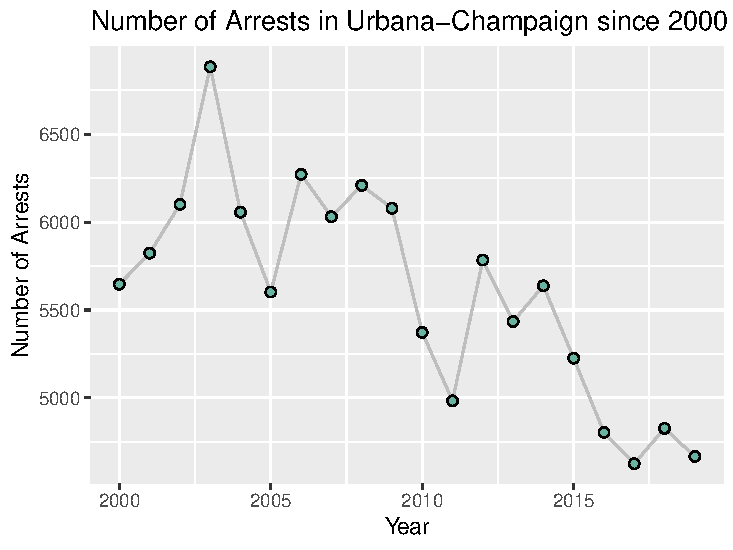
\includegraphics{progress-report_files/figure-pdf/unnamed-chunk-5-1.pdf}

}

\end{figure}

Based on this graph, we can see that 2003 has the highest number of
arrests from 2000 to 2023. Moreover, there is a decreasing trend on
number of arrests through out years.

\begin{verbatim}
# Graph to see in each year arrestees sex proportion
my_data %>% 
  ggplot(aes(x = year_of_arrest, fill = arrestee_sex)) +
  geom_histogram(binwidth = 0.5, color="#e9ecef", alpha=0.9) +
  ggtitle("Arrestee Sex in Urbana-Champaign since 2000") +
  labs(x = "Year", y = "Number of Arrests")
\end{verbatim}

\begin{figure}[H]

{\centering 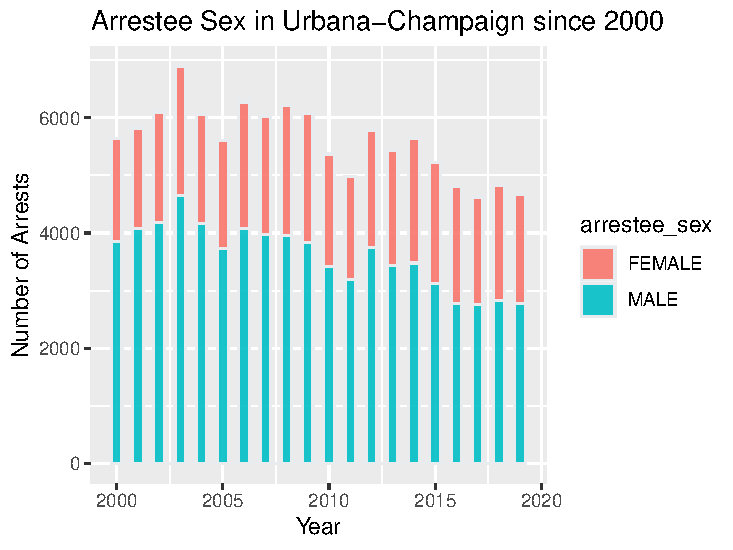
\includegraphics{progress-report_files/figure-pdf/unnamed-chunk-6-1.pdf}

}

\end{figure}

Based on this graph, we can see that Male contributes over 50\% of
arrests each year, which means that MALE is more likely to got arrested
compared with FEMALE.

\begin{verbatim}
# Graph to see in each year arrestee race proportion
my_data %>% 
  ggplot(aes(x = year_of_arrest, fill = arrestee_race)) +
  geom_histogram(binwidth = 0.5, color="#e9ecef", alpha=0.9) +
  ggtitle("Arrestee Race in Urbana-Champaign since 2000") +
  labs(x = "Year", y = "Number of Arrests")
\end{verbatim}

\begin{figure}[H]

{\centering 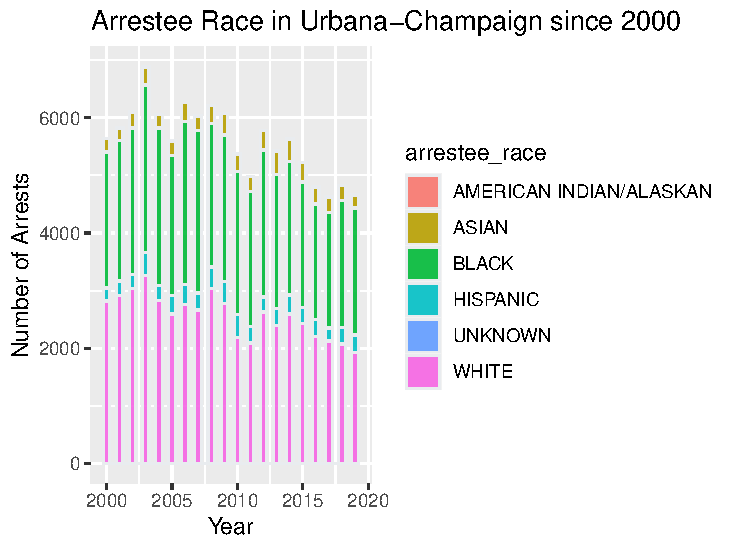
\includegraphics{progress-report_files/figure-pdf/unnamed-chunk-7-1.pdf}

}

\end{figure}

Based on this graph, we can see there BALCK and WHITE contribute over
80\% arrests. We can roughly see that WHITE contributes a little more
than BLACK.

\begin{verbatim}
# Check CHAMPAIGN spelling
unique(str_extract_all(my_data$arrestee_home_city, pattern = "\\bCHAMPA\\w*", simplify = TRUE))
\end{verbatim}

\begin{verbatim}
      [,1]        
 [1,] ""          
 [2,] "CHAMPAIGN" 
 [3,] "CHAMPAING" 
 [4,] "CHAMPAGIN" 
 [5,] "CHAMPAAIGN"
 [6,] "CHAMPAIGNN"
 [7,] "CHAMPAIGH" 
 [8,] "CHAMPAIG"  
 [9,] "CHAMPAGN"  
[10,] "CHAMPAIGGN"
\end{verbatim}

\begin{verbatim}
## Check URBANA spelling
unique(str_extract_all(my_data$arrestee_home_city, pattern = "\\bURBA\\w*", simplify = TRUE))
\end{verbatim}

\begin{verbatim}
     [,1]       
[1,] "URBANA"   
[2,] ""         
[3,] "URBAAN"   
[4,] "URBANDALE"
[5,] "URBANQA"  
[6,] "URBANAI"  
[7,] "URBAN"    
\end{verbatim}

\begin{verbatim}
## Replace wrong spelling
my_data$arrestee_home_city = str_replace_all(my_data$arrestee_home_city, pattern = "\\bCHAMPA\\w*", replacement = "CHAMPAIGN")
my_data$arrestee_home_city = str_replace_all(my_data$arrestee_home_city, pattern = "URBAAN", replacement = "URBANA")
my_data$arrestee_home_city = str_replace_all(my_data$arrestee_home_city, pattern = "URBANQA", replacement = "URBANA")
my_data$arrestee_home_city = str_replace_all(my_data$arrestee_home_city, pattern = "URBANAI", replacement = "URBANA")
my_data$arrestee_home_city = str_replace_all(my_data$arrestee_home_city, pattern = "URBAN", replacement = "URBANA")
my_data$arrestee_home_city = str_replace_all(my_data$arrestee_home_city, pattern = "URBANAA", replacement = "URBANA")

# mutate a column specify Champaign or Urbana or other home cities.
my_data %>% 
  mutate(homecity = ifelse((arrestee_home_city == "CHAMPAIGN" | arrestee_home_city == "URBANA"), arrestee_home_city, "OTHERS" )) %>% 
## Graph to show proportions of arrestee home city in each year
  ggplot(aes(x = year_of_arrest, fill = homecity)) +
  geom_histogram(binwidth = 0.5, color="#e9ecef", alpha=0.9) +
  ggtitle("Arrestee Home City in Urbana-Champaign since 2000") +
  labs(x = "Year", y = "Number of Arrests")
\end{verbatim}

\begin{figure}[H]

{\centering 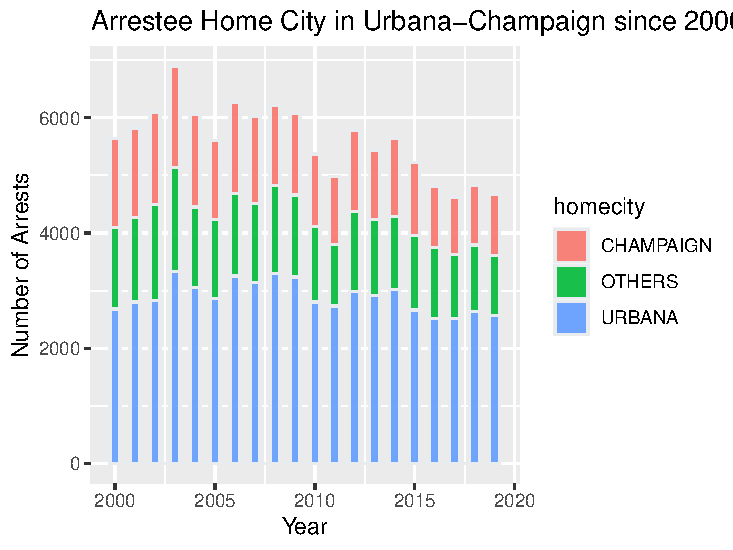
\includegraphics{progress-report_files/figure-pdf/unnamed-chunk-8-1.pdf}

}

\end{figure}

Based on this graph, we can see that most arrestees are from URBANA.
Arrestess from CHAMPAIGN and Other home cities roughtly contribute the
same to the total number of arrests in each year.

\hypertarget{time-line}{%
\subsection{Time Line}\label{time-line}}

\begin{figure}[H]

{\centering 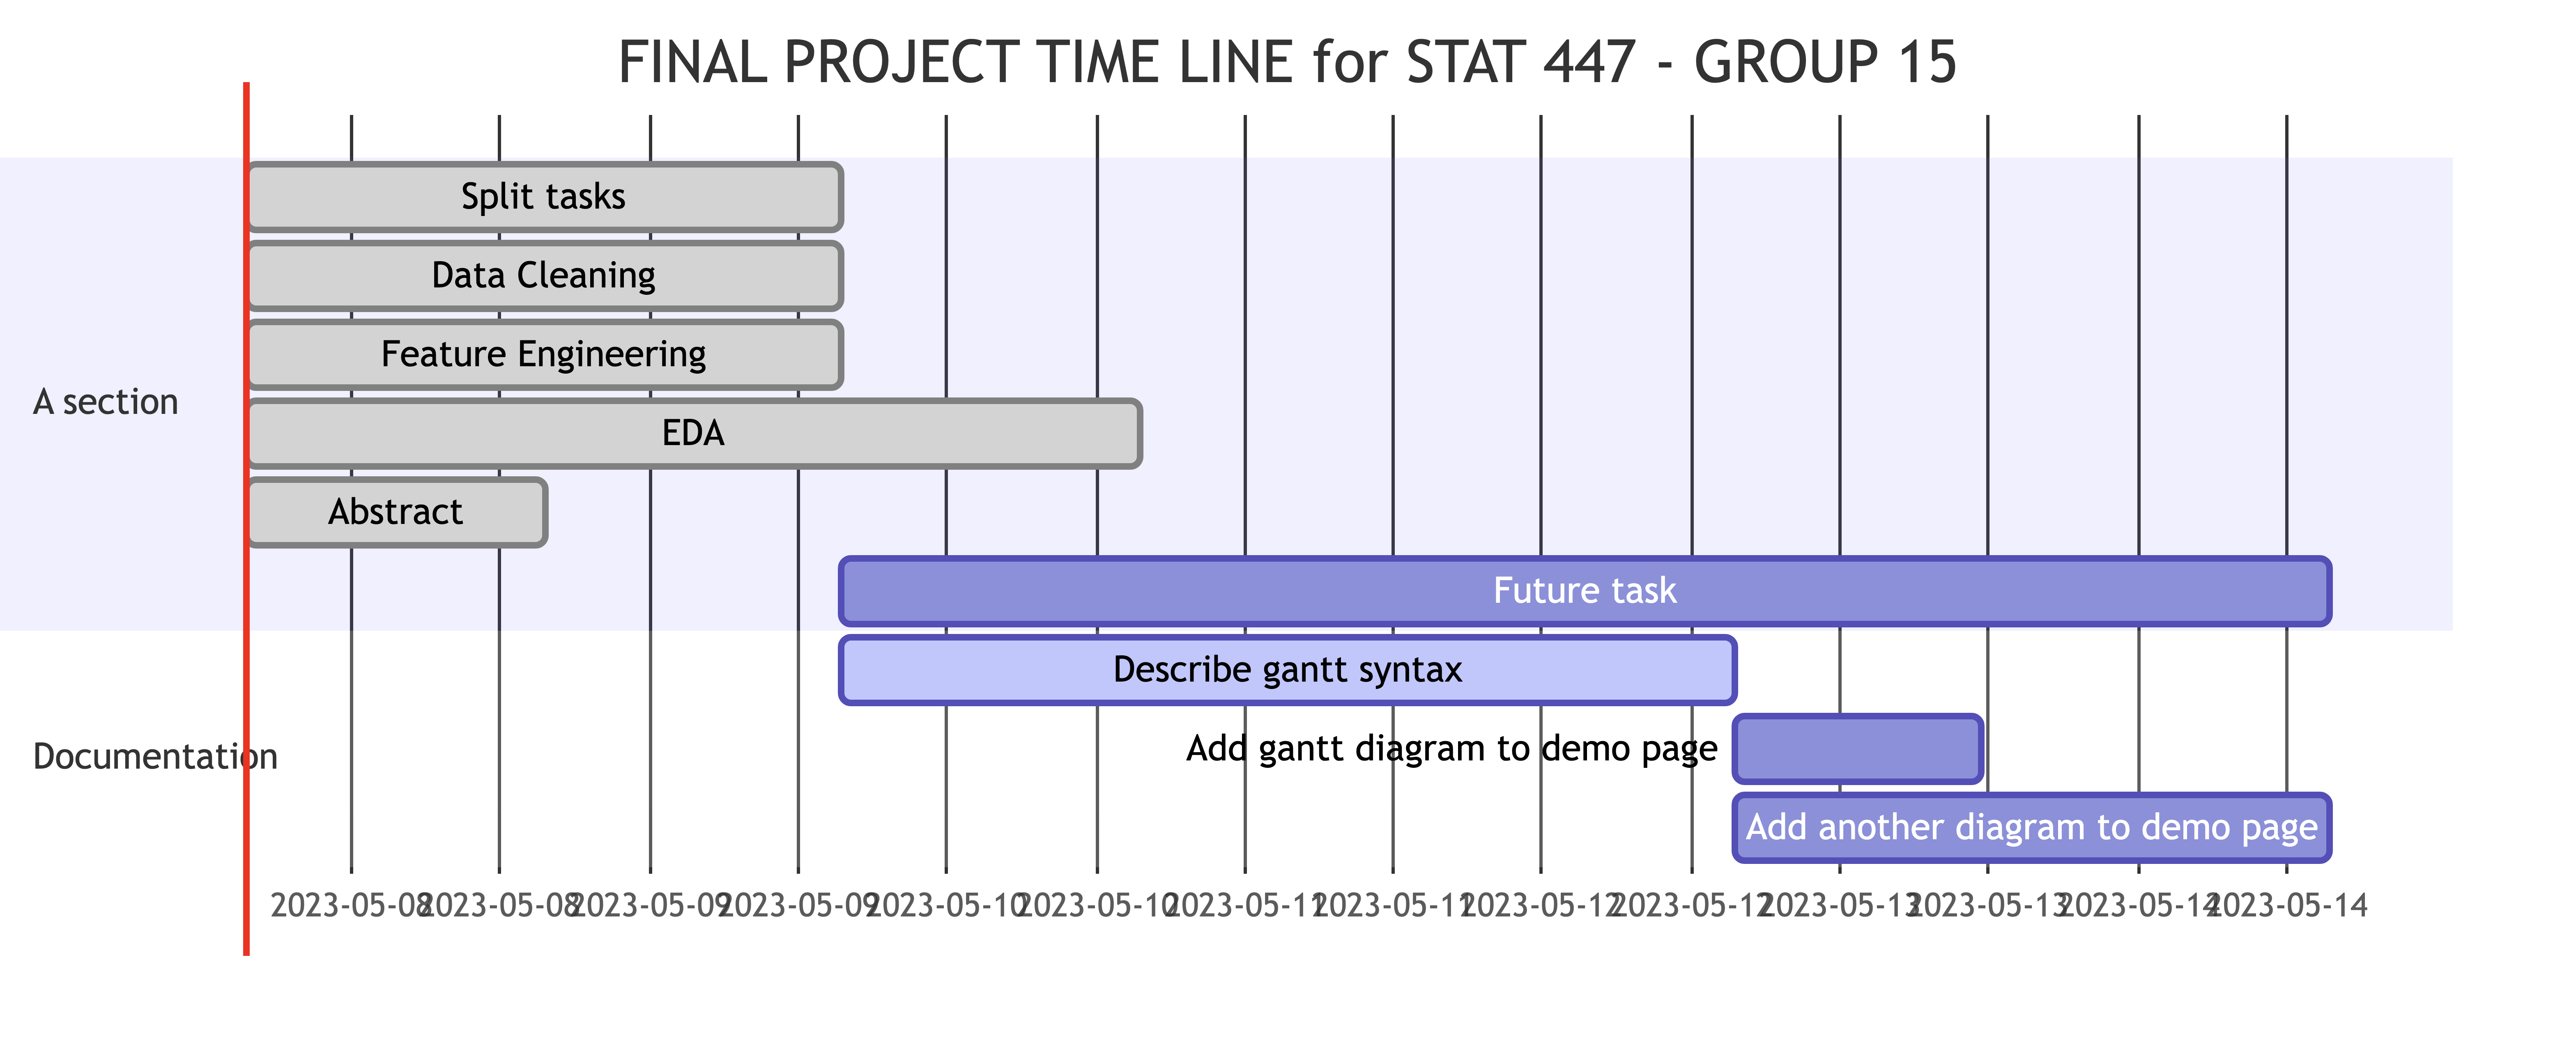
\includegraphics[width=8.17in,height=3.29in]{progress-report_files/figure-latex/mermaid-figure-1.png}

}

\end{figure}

\hypertarget{contribution}{%
\section{Contribution}\label{contribution}}

Xiangyu Jin is responsible for Explanatory Data Analysis: 50\%

Vinayak Bagdi is responsible for Abstract, Introduction and Related
Works: 50\%


  \bibliography{bibliography.bib}


\end{document}
